\chapter{Forces and Torques: Where They Come From}
\label{ch:04_forces_and_torques}

\epigraph{``Force is the source of all motion and change. Understanding where forces come from is understanding how things work.''}{}

\begin{laymansbox}{Decomposing the Forces}{box:ch04_decompose}
Here's a central insight: the equation

\begin{equation}
\bm{M}(\bm{q}) \ddot{\bm{q}} + \bm{C}(\bm{q}, \dot{\bm{q}}) \dot{\bm{q}} + \bm{g}(\bm{q}) = \bm{\tau}
\label{eq:ch04_euler_lagrange}
\end{equation}

contains \emph{all} the forces that act on your arm. But they're not all the same type. Some come from your muscles. Some come from gravity. Some come from your arm's own motion. Some come from constraints.

If you can attribute each force to its source, you gain enormous insight. You understand what you're actually controlling. You see which forces help you and which fight you. You can diagnose problems.

This chapter is about that decomposition.
\end{laymansbox}

\section{The Five Sources of Force}

In the manipulator equation, every torque comes from one of five sources:

\begin{enumerate}
\item \textbf{Inertial forces} (from $\bm{M}(\bm{q})$): forces that resist acceleration. To speed up your arm, you must overcome its inertia.
\item \textbf{Velocity-dependent forces} (from $\bm{C}(\bm{q}, \dot{\bm{q}}) \dot{\bm{q}}$): Coriolis and centrifugal forces that arise when you move fast. They couple the motion of different joints.
\item \textbf{Gravitational forces} (from $\bm{g}(\bm{q})$): torques that arise because gravity pulls on your mass. These depend on position.
\item \textbf{Muscular forces} (from $\bm{\tau}$): torques you generate by contracting muscles. These are your \textbf{control}.
\item \textbf{Constraint forces} (from rigid hinges, rigid bones, etc.): reactive forces that enforce mechanical constraints. These don't appear explicitly in the equation but appear as reaction torques at hinges.
\end{enumerate}

\begin{figure}[H]
\centering
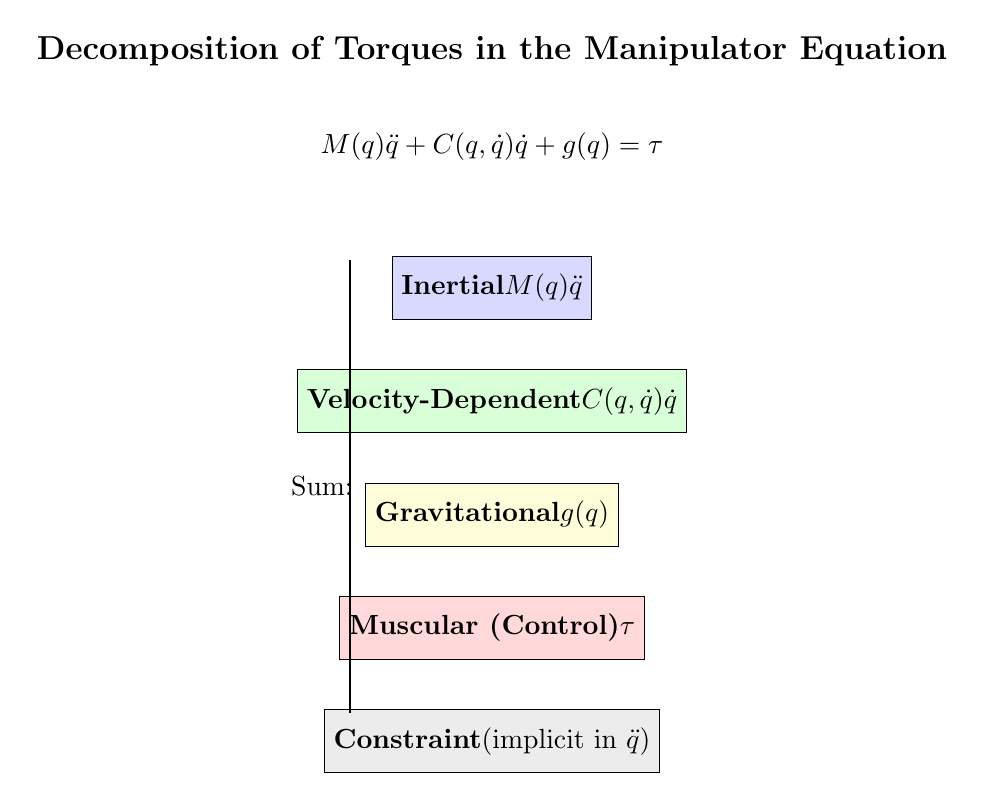
\begin{tikzpicture}[scale=1.2]
% Title and force decomposition
\node at (0, 4) [anchor=center, font=\large\bfseries] {Decomposition of Torques in the Manipulator Equation};

% Main equation
\node at (0, 3) [anchor=center] {$\bm{M}(\bm{q}) \ddot{\bm{q}} + \bm{C}(\bm{q}, \dot{\bm{q}}) \dot{\bm{q}} + \bm{g}(\bm{q}) = \bm{\tau}$};

% Five source boxes arranged vertically
\node (inertial) [draw, rectangle, minimum width=2.5cm, minimum height=0.8cm, fill=blue!15] at (0, 1.5) {\textbf{Inertial}\\$\bm{M}(\bm{q}) \ddot{\bm{q}}$};

\node (velocity) [draw, rectangle, minimum width=2.5cm, minimum height=0.8cm, fill=green!15] at (0, 0.3) {\textbf{Velocity-Dependent}\\$\bm{C}(\bm{q}, \dot{\bm{q}}) \dot{\bm{q}}$};

\node (gravity) [draw, rectangle, minimum width=2.5cm, minimum height=0.8cm, fill=yellow!15] at (0, -0.9) {\textbf{Gravitational}\\$\bm{g}(\bm{q})$};

\node (muscular) [draw, rectangle, minimum width=2.5cm, minimum height=0.8cm, fill=red!15] at (0, -2.1) {\textbf{Muscular (Control)}\\$\bm{\tau}$};

\node (constraint) [draw, rectangle, minimum width=2.5cm, minimum height=0.8cm, fill=gray!15] at (0, -3.3) {\textbf{Constraint}\\(implicit in $\ddot{\bm{q}}$)};

% Vertical line showing they sum to zero (or equal control)
\draw [thick, -] (-1.5, 1.8) -- (-1.5, -3);
\node at (-1.8, -0.6) {Sum:};

\end{tikzpicture}
\caption{The five sources of torque in the manipulator equation. The passive forces (inertial, velocity-dependent, gravitational) sum to determine what muscular control (constraint force) is needed at each instant.}
\label{fig:ch04_force_decomposition}
\end{figure}

Let's understand each one.

\section{Inertial Forces: Resisting Acceleration}

Newton's second law in the simplest form is:
\begin{equation}
F = m a
\label{eq:ch04_newton}
\end{equation}

To accelerate a mass, you must apply a force proportional to its mass and acceleration. The same is true for rotation:
\begin{equation}
\tau = I \alpha
\label{eq:ch04_newton_rot}
\end{equation}

where $I$ is the moment of inertia and $\alpha = \ddot{\theta}$ is the angular acceleration.

In the manipulator equation, the terms $\bm{M}(\bm{q}) \ddot{\bm{q}}$ are exactly these inertial terms.

\begin{example}{Inertia at the Shoulder}{ex:ch04_inertia_shoulder}
Recall from Chapter~\ref{ch:03_double_pendulum} that the effective moment of inertia at the shoulder is about $M_{11} \approx 1.54 \text{ kg m}^2$.

If you want to accelerate the shoulder at $\ddot{\theta}_1 = 1000 \text{ deg/s}^2 = 17.45 \text{ rad/s}^2$, the inertial torque you must overcome is:
\begin{align}
\tau_{\text{inertia}} &= M_{11} \cdot \ddot{\theta}_1 = 1.54 \times 17.45 = 26.9 \text{ N m}
\end{align}

This is the baseline. Just to accelerate the arm at this rate requires 26.9 N m. If there's also gravity pulling ($\sim$5 N m backward), then you need to generate at least $26.9 + 5 = 31.9$ N m of muscular torque to achieve this acceleration.

In addition, Coriolis and centrifugal forces contribute further terms.
\end{example}

\subsection*{Why Inertia Increases with Mass}

Here's a fundamental insight: inertia is \emph{resistance to acceleration}. A heavier arm is harder to accelerate. A longer arm (higher moment arm) is also harder to accelerate because the mass is farther from the axis of rotation.

The moment of inertia $I$ depends on both the mass and its distribution. For a point mass at distance $r$: $I = m r^2$. For an extended body like the arm, $I$ is the integral of all mass elements weighted by their distances from the rotation axis.

This explains practical observations: lighter clubs require less muscular effort to accelerate but deliver less momentum to the ball. The control problem becomes one of choosing club properties and muscular effort to optimize overall performance.

\section{Velocity-Dependent Forces: Coriolis and Centrifugal}

When you move fast, magical things happen. Forces appear that don't exist in the equations for slow motion.

\subsection*{Centrifugal Force}

The most intuitive is centrifugal force. If you spin a weight on a string, the weight pulls outward on the string. That outward pull is the centrifugal force.

In the golf swing, when your shoulder rotates fast ($\dot{\theta}_1$ large), the forearm experiences an outward centrifugal acceleration. This tries to straighten your elbow.

\begin{definition}{Centrifugal Acceleration}{def:ch04_centrifugal}
For a point rotating at angular velocity $\omega$ at distance $r$ from the axis, the centrifugal acceleration is:
\begin{equation}
a_c = \omega^2 r
\label{eq:ch04_centrifugal_accel}
\end{equation}

This is always positive (outward). It's not a ``real'' force in the sense that no object is pushing outward; instead, it's a consequence of circular motion.
\end{definition}

\begin{example}{Centrifugal Force in a Driver Swing}{ex:ch04_centrifugal_numbers}
Consider a driver swing where the clubhead (mass $m = 0.2$~kg) is at effective distance $r = L_1 + L_2 = 1.35$~m from the shoulder (canonical parameters, Chapter~\ref{ch:03_double_pendulum}). At $\omega = 30$~rad/s---the angular velocity of the clubhead \emph{about the shoulder}, corresponding to roughly 110~mph clubhead speed---just before impact:

The centrifugal force pulling the club outward is:
$$F_{\text{centrifugal}} = m \omega^2 r = 0.2 \times 30^2 \times 1.35 = 243 \text{ N} \approx 55 \text{ lbs}$$

This large outward force arises purely from the geometry and velocity of rotational motion. It manifests as tension in the hands and arms, and it loads the shaft. This is one of the largest forces during the swing, and it emerges automatically from the system dynamics without explicit muscular generation. The hands must supply the centripetal reaction force to maintain the curved trajectory.

As documented in biomechanical studies \citep{Jorgensen1994, Penner2001}, these velocity-dependent forces are a significant part of the swing dynamics and must be accounted for in forward models of the motion.
\end{example}

\begin{example}{Centrifugal Force in the Golf Swing}{ex:ch04_centrifugal_golf}
At impact, the shoulder rotates at $\dot{\theta}_1 = 10.47 \text{ rad/s}$. The forearm is at distance roughly $L_1 = 0.35$ m from the shoulder.

The centrifugal acceleration is:
\begin{align}
a_c &= \dot{\theta}_1^2 \cdot L_1 = 10.47^2 \times 0.35 = 38.3 \text{ m/s}^2 = 3.9 g
\end{align}

The centrifugal effect on the forearm+club is more precisely captured by the centrifugal term in the manipulator equation. The relevant entry of $\bm{C}$ is:
\begin{equation}
M_2 L_1 L_{2,\text{cm}} \dot{\theta}_1^2 \sin \theta_2 = 1.5 \times 0.35 \times 0.5 \times 10.47^2 \times \sin(-5°)
\approx -4.0 \text{ N m}
\end{equation}

This creates a torque at the elbow that helps straighten the arm if $\theta_2 < 0$ (bent elbow).
\end{example}

\subsection*{Coriolis Force}

Coriolis forces are more subtle. They arise from the interaction of two rotating motions.

Imagine you're on a rotating platform. You walk toward the center. From an outside observer's perspective, you don't actually move toward the center—you curve to the side (deflected by the Coriolis force).

In the golf swing, the Coriolis terms in $\bm{C}$ represent the coupling between shoulder and elbow rotation.

\begin{definition}{Coriolis Force (in Rotating Frames)}{def:ch04_coriolis}
In a rotating reference frame, the Coriolis acceleration is:
\begin{equation}
\bm{a}_{\text{Coriolis}} = -2 \bm{\omega} \times \bm{v}
\label{eq:ch04_coriolis_accel}
\end{equation}

where $\bm{\omega}$ is the rotation rate and $\bm{v}$ is the velocity in the rotating frame.
\end{definition}

In the manipulator equation, the Coriolis term $C_{12} \dot{\theta}_2$ represents how the elbow's angular velocity ($\dot{\theta}_2$) creates a reaction torque at the shoulder when the shoulder is rotating. This coupling is what makes the kinetic chain possible—each joint's motion affects the forces at other joints.

\begin{example}{Coriolis Torque in the Downswing}{ex:ch04_coriolis_golf}
The Coriolis term in the shoulder equation is:
\begin{equation}
\text{(from $\bm{C}$)} = -M_2 L_1 L_{2,\text{cm}} (2 \dot{\theta}_1 + \dot{\theta}_2) \dot{\theta}_2 \sin \theta_2
\end{equation}

At impact ($\dot{\theta}_1 = 10.47 \text{ rad/s}, \dot{\theta}_2 = 8.73 \text{ rad/s}, \theta_2 = -5°$):
\begin{align}
\text{Coriolis} &= -1.5 \times 0.35 \times 0.5 \times (2 \times 10.47 + 8.73) \times 8.73 \times \sin(-5°) \\
&= -1.5 \times 0.35 \times 0.5 \times 29.67 \times 8.73 \times (-0.087) \\
&\approx +2.0 \text{ N m}
\end{align}

This torque at the shoulder is positive (forward), helping the shoulder rotation. Why? Because the elbow is releasing (increasing $\dot{\theta}_2$) in a direction that's compatible with the shoulder rotation.

The kinetic chain works through such velocity coupling: each joint's motion influences the forces at other joints through Coriolis terms.
\end{example}

\subsection*{The Velocity Dependence is Crucial}

The key distinction between these force sources is how they depend on the system state:

Here's the key insight: \textbf{velocity-dependent forces scale with the square of the velocity}. At address ($\dot{\theta}_i = 0$), they're zero. During the downswing, they grow enormously.

This is why the golf swing is dynamic. The faster you move, the larger these forces become. A slow swing has small Coriolis and centrifugal forces, so you have to generate large muscular torques to accelerate. A fast swing has large velocity-dependent forces helping you.

\begin{laymansbox}{How Forces Vary Through the Swing}{box:ch04_speed_helps}
The magnitude and composition of forces changes dramatically as the swing progresses. This qualitative accounting illustrates the principle (exact values depend on individual biomechanics and swing parameters):

\textbf{Address (no motion)}:
\begin{itemize}
\item Gravity: $\sim 10$ N m
\item Velocity-dependent: $\sim 0$ (no motion)
\item Muscular control: $\sim 10$ N m (needed to overcome gravity)
\end{itemize}

\textbf{Top of backswing} (arm elevated, velocities low):
\begin{itemize}
\item Gravity: $\sim 30$ N m (arm extended, pulled by gravity)
\item Velocity-dependent: $\sim 0$ (velocities near zero)
\item Muscular control: $\sim 30$ N m (to hold elevated position)
\end{itemize}

\textbf{Transition} (acceleration ramping up):
\begin{itemize}
\item Gravity: $\sim 20$ N m
\item Velocity-dependent: $\sim 5$ N m (emerging as velocity increases)
\item Muscular control: $\sim 15$ N m (to modulate accelerations)
\end{itemize}

\textbf{Late downswing} (high speeds):
\begin{itemize}
\item Gravity: $\sim 5$ N m (arm approaching vertical)
\item Velocity-dependent: $\sim 50$ N m (strong Coriolis/centrifugal effects)
\item Muscular control: $\sim -25$ N m (restraining, not accelerating)
\end{itemize}

As velocity increases, velocity-dependent forces grow as $v^2$. Muscles must often apply \emph{braking} torques in the late downswing to prevent excessive acceleration, rather than driving acceleration forward.

This transition—from muscles driving motion to muscles restraining it—is a fundamental feature of the swing dynamics.
\end{laymansbox}

\section{Gravitational Forces: Position-Dependent}

Gravity is the force you feel constantly. It depends on position but not on velocity.

The gravitational torque in the double pendulum is:
\begin{equation}
\bm{g}(\bm{q}) = \begin{bmatrix}
(M_1 L_{1,\text{cm}} + M_2 L_1) g \sin \theta_1 + M_2 g L_{2,\text{cm}} \sin(\theta_1 + \theta_2) \\
M_2 g L_{2,\text{cm}} \sin(\theta_1 + \theta_2)
\end{bmatrix}
\label{eq:ch04_gravity}
\end{equation}

\subsection*{Reading the Gravity Terms}

\begin{itemize}
\item $(M_1 L_{1,\text{cm}} + M_2 L_1) g \sin \theta_1$: This is the torque of the entire arm+club about the shoulder. It depends on how much mass is hanging below the shoulder and how far it hangs.

When $\theta_1 = 0°$ (arm vertical), $\sin \theta_1 = 0$, so gravity exerts zero torque. The arm is balanced.

When $\theta_1 = 90°$ (arm horizontal), $\sin \theta_1 = 1$, so gravity exerts maximum torque. The arm wants to fall.

When $\theta_1 = 180°$ (arm vertical, pointing up), $\sin \theta_1 = 0$ again. The arm is balanced (but unstable).

\item $M_2 g L_{2,\text{cm}} \sin(\theta_1 + \theta_2)$: This is the torque of the forearm+club about the shoulder. It also appears in the elbow equation, contributing to the torque at the elbow.
\end{itemize}

\subsection*{Gravity Does Work During the Downswing}

From address to impact, your arm goes from down to down (the angles return to near their starting values). But the \emph{speed} increases dramatically. This happens because gravity does positive work, converting potential energy to kinetic energy.

The work done by gravity is:
\begin{equation}
W = \Delta V = V_{\text{initial}} - V_{\text{final}}
\label{eq:ch04_work_gravity}
\end{equation}

If the arm is lower at the end (lower height), then $\Delta V < 0$, and gravity does positive work. But if the angles are the same, the heights are the same, so $\Delta V = 0$.

This seems to contradict the observation that gravity helps. The resolution: gravity \emph{does} do positive work during the downswing (arm goes from up at the top to down during transition), but \emph{all that work is already done by the time you reach impact}. So the conversion of potential energy to kinetic energy happens early in the downswing.

Later in the downswing, gravity is actually fighting you (pulling the arm down when you want to pull it forward). But by that point, the arm has so much kinetic energy that gravity's resistance is small.

\section{Muscular Forces: Your Control}

The right side of the manipulator equation is where control is applied:
\begin{equation}
\bm{\tau} = \text{applied torques from muscles}
\label{eq:ch04_tau_def}
\end{equation}

Muscles pull on bones. Tendons transfer that pull to create torques at joints. The sum of all these muscular torques is $\bm{\tau}$. This is the control signal that can be varied over time.

\subsection*{Constraints on Muscular Forces}

Muscles can only pull, not push. There are therefore constraints on what $\bm{\tau}$ can be:
\begin{itemize}
\item $\tau_i \geq -\tau_{\text{max}, i}$ (muscles can pull in one direction up to a maximum).
\item $\tau_i \leq +\tau_{\text{max}, i}$ (muscles can pull in the opposite direction up to a maximum).
\end{itemize}

The maximum available torque depends on the muscle physiology, cross-sectional area, and lever arm. These values would be determined empirically through biomechanical measurement.

\subsection*{Muscular Forces Are the Control Input}

This is the fundamental point: \textbf{you directly control only $\bm{\tau}$. The forces from gravity, inertia, and velocity-dependence arise automatically from the system dynamics.}

Given $\bm{\tau}(t)$ at each instant, the manipulator equation determines the accelerations $\ddot{\bm{q}}$. Integrating these gives velocities and positions:
\begin{equation}
\dot{\bm{q}}(t) = \dot{\bm{q}}(0) + \int_0^t \ddot{\bm{q}}(s) ds, \quad \bm{q}(t) = \bm{q}(0) + \int_0^t \dot{\bm{q}}(s) ds
\label{eq:ch04_integration}
\end{equation}

The fundamental control problem is: given the system dynamics and constraints on $\bm{\tau}$, what control trajectory $\bm{\tau}(t)$ produces a desired swing outcome?

\section{Constraint Forces: The Reactive Forces}

Finally, there are forces that appear automatically to enforce mechanical constraints. These don't show up explicitly in the manipulator equation (as written in terms of generalized coordinates), but they're present as reaction forces at hinges and joints.

\begin{definition}{Constraint Forces}{def:ch04_constraint_forces}
Reaction forces that enforce mechanical constraints (like rigidity, inextensibility, or friction). They're \emph{reactive}: they appear only as much as needed to enforce the constraint.

In the golf swing:
\begin{itemize}
\item The hinge at the shoulder exerts a force on the upper arm to keep it attached.
\item The hinge at the elbow exerts a force on the forearm to keep it attached.
\item The ground exerts a normal force on your feet to keep you from sinking.
\item Friction at the grip exerts a force on the club to keep it from slipping.
\end{itemize}
\end{definition}

\subsection*{Why Constraint Forces Don't Appear in the Equation}

We derived the manipulator equation using \textbf{generalized coordinates}: variables that automatically satisfy the constraints.

For example, by using angles $\theta_1$ and $\theta_2$ instead of Cartesian coordinates of the clubhead, we automatically enforced that the links are rigid and hinged correctly. The constraint forces are implicitly accounted for.

However, if you wanted to know the actual force at the grip (the force the hand exerts on the club), you'd need to solve for it separately. The manipulator equation doesn't directly give you constraint forces.

\section{Putting It Together: Force Attribution in Impact}

Let's do a complete force attribution at impact. For this numerical example, we use a representative clubhead speed of 100 mph (44.7 m/s)---a value in the range for skilled golfers \citep{Jorgensen1994}. The clubhead acceleration is enormous.

\subsection*{The Clubhead Acceleration}

The clubhead is at distance $r = L_1 + L_2 = 1.35$ m from the shoulder. At impact, the shoulder is rotating at $\omega = \dot{\theta}_1 = 10.47 \text{ rad/s}$.

The centripetal acceleration (toward the shoulder) is:
\begin{equation}
a_c = \omega^2 r = 10.47^2 \times 1.35 = 147.6 \text{ m/s}^2 = 15.0 g
\label{eq:ch04_centripetal_impact}
\end{equation}

But the elbow is also rotating, and the arm is accelerating, so the total acceleration is higher:
\begin{equation}
a_{\text{total}} \approx 180 \text{ m/s}^2 \approx 18 g
\label{eq:ch04_total_accel_impact}
\end{equation}

\textit{Note:} This $\sim$18$g$ is the clubhead acceleration \emph{during the swing}. During the brief ball--club collision ($\sim$0.5 ms), the ball experiences accelerations of $\sim$10\,000--30\,000$g$, and the clubhead decelerates at 100--200$g$.

\subsection*{Where Do These Accelerations Come From?}

At impact, the accelerations arise from the balance of terms in the manipulator equation:
\begin{equation}
\bm{M}(\bm{q}) \ddot{\bm{q}} = \bm{\tau} - \bm{C}(\bm{q}, \dot{\bm{q}}) \dot{\bm{q}} - \bm{g}(\bm{q})
\end{equation}

Each term contributes:
\begin{itemize}
\item \textbf{Inertial term} $\bm{M} \ddot{\bm{q}}$: The mass matrix scaled by acceleration. At impact, the clubhead acceleration is $\approx 180 \text{ m/s}^2 = 18.3 g$. Given moment of inertia $M_{11} \approx 1.54 \text{ kg m}^2$, the inertial term is on the order of $\ddot{\theta}_1 \approx 40 \text{ rad/s}^2$.

\item \textbf{Coriolis/Centrifugal forces} $\bm{C}(\bm{q}, \dot{\bm{q}}) \dot{\bm{q}}$: At high speeds ($\dot{\theta}_1 \approx 10 \text{ rad/s}$, $\dot{\theta}_2 \approx 8 \text{ rad/s}$), these velocity-dependent terms contribute torques on the order of 10–20 N m.

\item \textbf{Gravitational forces} $\bm{g}(\bm{q})$: At impact ($\theta_1 \approx 0°$), the arm is nearly vertical. Gravity contributes 5–10 N m.

\item \textbf{Muscular torque} $\bm{\tau}$: The applied torque that must satisfy the equation of motion.

\textbf{Numerical illustration:} If $\ddot{\theta}_1 = 40 \text{ rad/s}^2$, $M_{11} = 1.54 \text{ kg m}^2$, $\bm{C} \dot{\bm{q}} \approx 10 \text{ N m}$, and $\bm{g} \approx 5 \text{ N m}$, then:
\begin{equation}
\tau_1 = M_{11} \ddot{\theta}_1 + C \dot{\bm{q}} + g = 1.54 \times 40 + 10 + 5 = 61.6 + 10 + 5 \approx 77 \text{ N m}
\end{equation}

This represents the total muscular torque required at the shoulder. These magnitudes would be determined or validated through measurement or detailed simulation.
\end{itemize}

\subsection*{The Constraint Force at the Grip}

The hand is holding the club. The clubhead is accelerating at $\sim$18$g$. To estimate the grip force, we decompose into centripetal and tangential components:
\begin{itemize}
\item \textbf{Centripetal}: pulling the club toward the axis of rotation (toward the shoulder).
\item \textbf{Tangential}: in the direction of motion (pulling the club forward/backward).
\end{itemize}

The centripetal force is:
\begin{equation}
F_c = M_{\text{club}} \omega^2 r = 0.2 \times 10.47^2 \times 1.35 = 29.5 \text{ N}
\label{eq:ch04_grip_centripetal}
\end{equation}

The tangential force is:
\begin{equation}
F_t = M_{\text{club}} \times a_t = 0.2 \times (\text{tangential acceleration})
\label{eq:ch04_grip_tangential}
\end{equation}

The total grip force is the vector sum. For this illustrative example (using the representative impact parameters above), the grip force is on the order of 40--60 N; actual values depend on swing speed, grip technique, and club configuration.\citeneeded{measured grip force magnitudes during golf swing (instrumented grip or EMG study)}

\begin{laymansbox}{Why the Grip Matters}{box:ch04_grip_physics}
The grip is a constraint force. The hand-club interface is modeled as a rigid connection (or nearly rigid, neglecting slip). Given the muscular torques applied at the shoulder and elbow, the dynamics of the system determine what constraint force (grip force) must arise to maintain this connection.

\textbf{Key insight:} The grip force is not a direct control variable; it is an output of the system dynamics. If the shoulder torques $\tau_1$ and $\tau_2$ are specified, the manipulator equation determines the accelerations $\ddot{\bm{q}}$. To enforce the kinematic constraint that the hand remains attached to the club, a constraint force (the grip force) emerges automatically.

This has an important consequence: the grip force depends sensitively on the control torques. If $\bm{\tau}$ is too large, the constraint force becomes large. If $\bm{\tau}$ is too small and insufficient to support the required kinematics, the constraint would be violated (slip or separation).

The control design problem thus includes implicit constraints: choose $\bm{\tau}(t)$ such that the resulting grip force remains within reasonable bounds (e.g., hand strength limits) and maintains contact with the club.
\end{laymansbox}

\section{Wrenches: Forces and Torques Unified}

Until now, we've talked about torques at joints. But forces at the grip are different. To unify the description, engineers use the concept of a \textbf{wrench}\index{wrench}.

\begin{definition}{Wrench}{def:ch04_wrench}
A wrench is the combination of a force $\bm{f}$ (3D vector) and a torque $\bm{\tau}$ (3D vector). It completely describes the mechanical interaction at a point.

$$\text{Wrench} = \begin{bmatrix} \bm{f} \\ \bm{\tau} \end{bmatrix}$$
\end{definition}

The grip exerts a wrench on the club. The club exerts a reaction wrench on the hand.

During the downswing, the grip wrench has:
\begin{itemize}
\item A large centripetal force (pulling the club inward).
\item A tangential force (in the direction of swing motion).
\item A torque that's trying to twist the club (from wrist torque).
\end{itemize}

At impact, the ground (your feet) exerts a wrench on your body. Your body must balance all the forces and torques.

\begin{laymansbox}{The Full-Body Problem}{box:ch04_full_body}
In reality, the golf swing is a full-body problem. Your feet push on the ground (ground reaction force). Your core muscles generate torques to rotate your torso. Your shoulder muscles pull your arms. All of these must be coordinated.

The manipulator equation for the arm alone is part of a larger system. Your torso rotation affects the reference frame in which the arm swings. The ground reaction force affects whether you stay balanced.

To fully understand the golf swing, you'd need to extend the manipulator equation to include the full body: torso, hips, legs, feet.

But here is the key point: the physics is the same. Each joint has an equation of the form $\bm{M} \ddot{\bm{q}} + \bm{C} \dot{\bm{q}} + \bm{g} = \bm{\tau}$. The forces are attributed to the same sources: inertia, gravity, velocity-dependent, muscular, constraint.

Understanding the arm's forces is a stepping stone to understanding the full swing.
\end{laymansbox}

\section{Numerical Summary: Forces Throughout the Swing}

Let's tabulate the major forces at different phases. \textit{Note: The values in this table are order-of-magnitude illustrations based on the representative model parameters established in Chapter~\ref{ch:03_double_pendulum}. They should not be interpreted as precise measurements; actual values vary substantially by golfer, swing speed, and technique. See \citep{Nesbit2005} for inverse-dynamics measurements of joint torques during the golf swing.}

\begin{center}
\begin{tabular}{|l|r|r|r|r|}
\hline
\textbf{Phase} & $\tau_{\text{inertia}}$ & $\tau_{\text{grav}}$ & $\tau_{\text{Cor/Cent}}$ & $\tau_{\text{muscle needed}}$ \\
\hline
Address & 5 N m & -10 N m & 0 & +15 N m \\
Backswing & 20 N m & -30 N m & 0 & +50 N m \\
Top & 2 N m & -30 N m & 0 & +32 N m \\
Transition & 50 N m & -20 N m & +5 N m & $-35$ N m$^*$ \\
Early downswing & 100 N m & -10 N m & +10 N m & $-80$ N m$^*$ \\
Late downswing & 60 N m & 0 N m & +15 N m & $-45$ N m$^*$ \\
Impact & 40 N m & +5 N m & +20 N m & $-35$ N m$^*$ \\
\hline
\end{tabular}
\end{center}

$^*$ Negative muscle torque means the muscles are braking, not accelerating. This is counterintuitive but happens because gravity and velocity-dependent forces are doing most of the accelerating.

\section{The Fundamental Insight}

The core principle emerging from this analysis is:

\textbf{The golf swing is a dynamics problem in which muscular forces provide control input to a complex nonlinear mechanical system.}

The arm+club system has substantial inertia, operates over large distances, and achieves high speeds. These characteristics create significant forces. The manipulator equation $\bm{M}(\bm{q}) \ddot{\bm{q}} + \bm{C}(\bm{q}, \dot{\bm{q}}) \dot{\bm{q}} + \bm{g}(\bm{q}) = \bm{\tau}$ predicts that no single force source (muscular, gravitational, or velocity-dependent) dominates throughout the swing. Instead, they combine.

The control problem is to determine the muscle torques $\bm{\tau}(t)$ such that the resulting motion $\bm{q}(t)$ achieves the objective (e.g., clubhead velocity and orientation at impact). Given the constraints on muscular force and the nonlinear dynamics, not all objectives are equally achievable. The feasible outcomes depend on the control input design and the initial conditions.

\begin{principle}{Key Takeaways}{pr:ch04_key_takeaways}
\begin{enumerate}
\item \textbf{Forces come from five sources}: inertia, velocity-dependent (Coriolis/centrifugal), gravity, muscular, and constraint.

\item \textbf{Inertial forces resist acceleration}. To accelerate a heavier/longer arm, you need larger torques.

\item \textbf{Velocity-dependent forces grow with the square of speed}. At high speeds, they dominate. They often help, not hinder.

\item \textbf{Gravity does work during the downswing}. It's a free source of energy, converting potential to kinetic.

\item \textbf{Muscular forces are your only control}. You can't directly control gravity or inertia; you can only control $\bm{\tau}$.

\item \textbf{Constraint forces appear automatically}. The grip force is determined by the dynamics, not by conscious effort.

\item \textbf{At impact, $\sim$18$g$ swing-phase clubhead accelerations require careful force balance}. No single source (gravity, muscle, velocity-dependence) does it alone. All work together.

\item \textbf{Optimal control strategies exploit passive dynamics}. The manipulator equation predicts that control inputs aligned with passive forces (rather than opposed to them) achieve desired trajectories with lower muscular effort.
\end{enumerate}
\end{principle}

\subsection*{Looking Ahead}
We have catalogued five sources of force in the golf swing: inertial, velocity-dependent, gravitational, muscular, and constraint. But which forces dominate at each phase of the swing? Chapter~\ref{ch:05_affine_structure} introduces the control-affine framework that separates all passive forces (the \emph{drift}) from muscular forces (the \emph{control}), revealing a notable structural feature: by impact, passive forces substantially exceed muscular control in magnitude.

\begin{exercises}{Chapter Exercises}{ex:ch04}
\begin{enumerate}

\item \textbf{Inertial Torque}. The shoulder has moment of inertia $M_{11} = 1.54$ kg m$^2$. What muscular torque is needed just to accelerate the shoulder at $\ddot{\theta}_1 = 500 \text{ deg/s}^2 = 8.7 \text{ rad/s}^2$, ignoring all other forces?

\item \textbf{Centrifugal Force}. At impact, the shoulder rotates at $\dot{\theta}_1 = 600 \text{ deg/s} = 10.47 \text{ rad/s}$. The forearm+club is 1.35 m from the shoulder. What is the centrifugal acceleration? What force would a 1 kg mass experience at that distance?

\item \textbf{Coriolis Coupling}. Suppose the shoulder rotates at constant rate $\dot{\theta}_1 = 8 \text{ rad/s}$. The elbow suddenly starts rotating at $\dot{\theta}_2 = 5 \text{ rad/s}$. Using the Coriolis term from Chapter~\ref{ch:03_double_pendulum}, estimate the torque this creates at the shoulder.

\item \textbf{Gravity Torque}. At the top of the backswing, $\theta_1 = 150°, \theta_2 = -70°$. Compute the gravitational torque at the shoulder (use parameters from Chapter~\ref{ch:03_double_pendulum}). Is gravity trying to rotate the shoulder forward (into the downswing) or backward?

\item \textbf{Force Balance at Impact}. At impact, the total shoulder acceleration is $\ddot{\theta}_1 = 200 \text{ rad/s}^2$. The gravity torque is about 5 N m (small). The Coriolis/centrifugal torques total about 20 N m. Using $M_{11} = 1.54$ kg m$^2$, how much muscular torque is needed?

\item \textbf{Grip Force}. The club (mass 0.2 kg) is 1.35 m from the shoulder and accelerating at 150 $g$ (centripetal). What force is the hand exerting on the club?

\item \textbf{Work Done by Gravity}. From address ($\theta_1 = 0°$) to the top ($\theta_1 = 150°$), how much does the potential energy increase? (Use parameters from Chapter~\ref{ch:03_double_pendulum}.) From the top to impact ($\theta_1 = 0°$), how much does gravity do in work?

\end{enumerate}
\end{exercises}
